\section{Analisi lineare}
Lo sviluppo tecnologico dei prodotti elettrodomestici si è tradotto, nel caso della lavatrice, in un incremento della velocità di rotazione, della capienza di cestello e una diminuzione del peso, in favore di un minor costo di impiego dei materiali. A causa di questi sviluppi, il problema delle vibrazioni risulta sempre più presente e la sua risoluzione acquisisce particolare interesse.

La seguente analisi tratta il modello più diffuso a livello europeo, ovvero la lavatrice a tamburo ad asse di rotazione orizzontale (Figura \ref{LavatriceAsseOrizzontale}).
\begin{figure}[h]
    \centering
    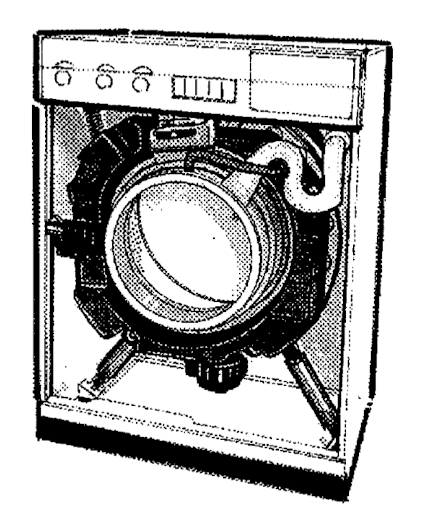
\includegraphics[scale=0.5]{LavatriceOrizzontale.png}
    \caption{Illustrazione di un modello di lavatrice ad asse orizzontale.}
    \label{LavatriceAsseOrizzontale}
\end{figure}\\
Se il modello dinamico di una lavatrice a tamburo viene semplificato, può essere convertito in un modello di rotore tridimensionale (Figura \ref{ModelloRotore})\cite{choi2003study}.
\begin{figure}[h]
    \centering
    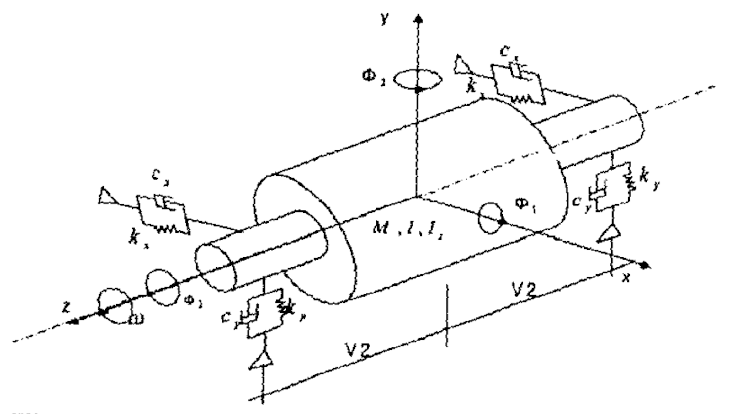
\includegraphics[scale=0.5]{ModelloRotore.png}
    \caption{Modello dinamico di una lavatrice a tamburo.}
    \label{ModelloRotore}
\end{figure}\\
Per comodità di analisi, supponendo che sia simmetrico rispetto all'asse y impostato, il problema si può ridurre ad un modello bi-dimensionale \cite{choi2003study}. 
A questo punto si avrà un'idea del modello teorico, il quale è stato trattato per dare un'ottica generale del caso pratico oggetto di studio.
\subsection{Modello bidimensionale}
Lo schema rappresentato in Figura \ref{Modello2D} vede il cestello perforato che contiene la biancheria posto all'interno di un involucro stagno, che contiene a sua volta acqua durante la fase di lavaggio, ed è vuoto durante la centrifugazione \cite{esercitazioneapplicata}.

Per assorbire l'effetto delle oscillazioni dovute allo sbilanciamento del carico durante la centrifugazione, è previsto un sistema di 3 molle e 3 smorzatori viscosi.
\begin{figure}[h]
    \centering
    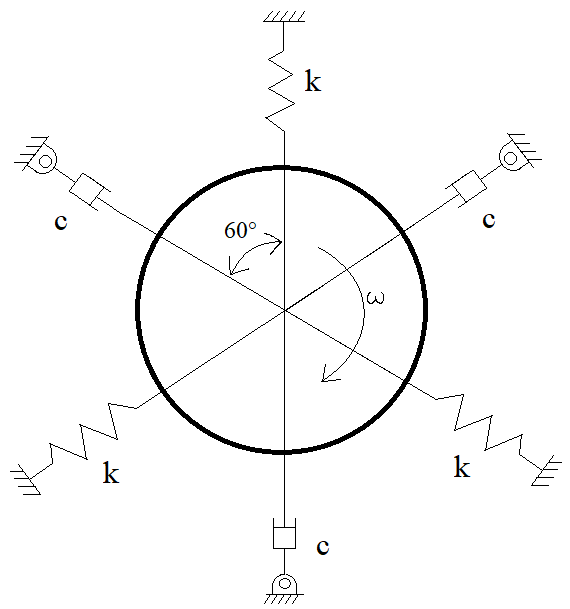
\includegraphics[scale=0.63]{Lavatrice3Smorz3Molle.png}
    \caption{Schematizzazione 2D del sistema lavatrice.}
    \label{Modello2D}
\end{figure}

I dati del problema sono:
\begin{itemize}
    \item \textbf{m} = massa della biancheria rotante attorno all'asse del cestello [kg];
    \item \textbf{M} = massa totale sospesa [kg];
    \item \textbf{e} = eccentricità massima delle masse rotanti [m];
    \item \textbf{n} = velocità di rotazione della centrifuga [rpm];
    \item \textbf{Costanti delle molle} = k [N/m];
    \item \textbf{Costanti degli smorzatori} = c [Ns/m].
\end{itemize}

Scegliamo un sistema di coordinate come mostrato in Figura \ref{SistemaCoordinate}.
\\
In un primo momento si considerano solo l'azione delle molle, ovvero la forza elastica da esse esercitata. 
Si considera un piccolo spostamento in direzione x. La molla 1 si allunga, la molla 3 si comprime e la molla 2 è soggetta ad una variazione di lunghezza trascurabile. 
\begin{figure}[h]
    \centering
    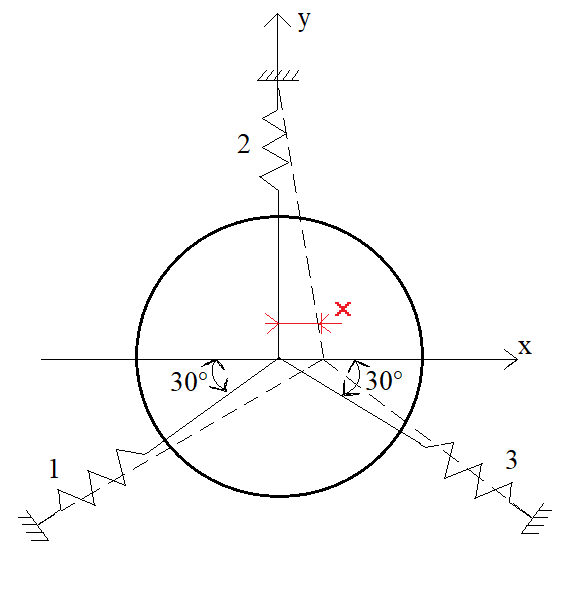
\includegraphics[scale=0.6]{Lavatrice3Molle.png}
    \caption{Sistema di coordinate e piccolo spostamento in direzione x.}
    \label{SistemaCoordinate}
\end{figure}

Le forze delle molle sono in prima approssimazione come indicato in Figura \ref{ForzeMolle}. La somma delle componenti verticali è nulla mentre si sommano le componenti orizzontali. 
\begin{figure}[h]
    \centering
    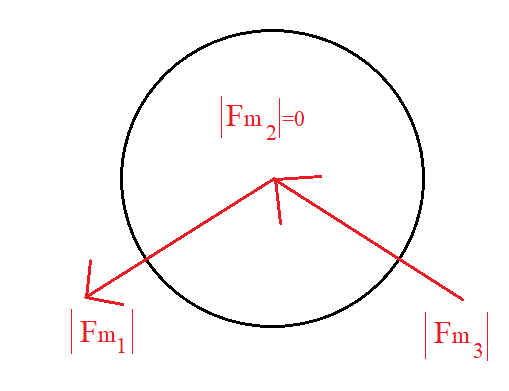
\includegraphics[scale=0.5]{LavatriceForze3Molle.png}
    \caption{Forze delle molle agenti sul cestello .}
    \label{ForzeMolle}
\end{figure}
\\
\begin{figure}[h]
    \centering
    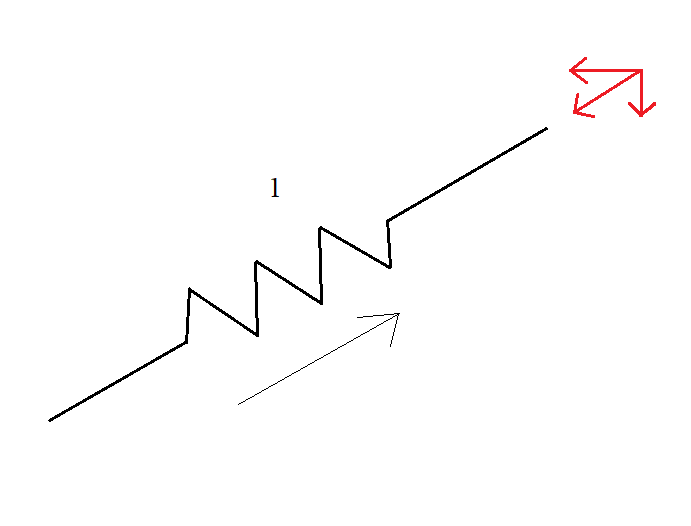
\includegraphics[scale=0.4]{Molla 1.png}
    \caption{Allungamento e forze molla 1.}
    \label{Molla1}
\end{figure}
\\
La molla 1 si allunga di $x\cos(30^\circ)$, il che implica una forza $F_{1}=k x\cos(30^\circ)$. La componente orizzontale di tale forza vale $F_{1}\cos(30^\circ)=k x\cos^2(30^\circ)$.
\\
\begin{figure}[h]
    \centering
    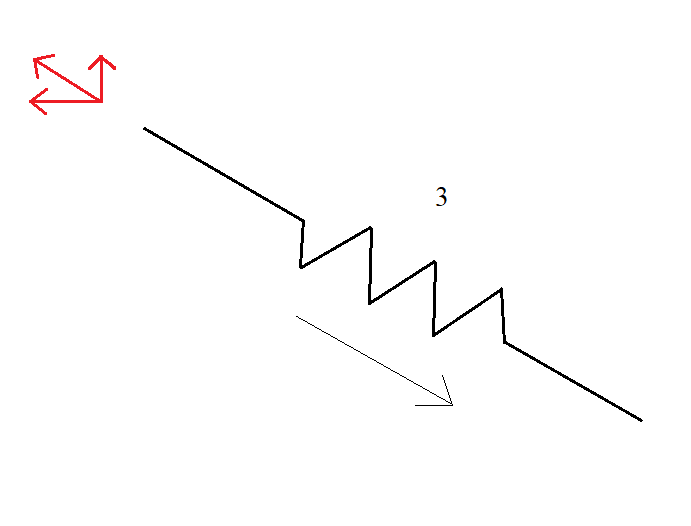
\includegraphics[scale=0.4]{Molla 3.png}
    \caption{Allungamento e forze molla 3.}
    \label{Molla3}
\end{figure}
\\
La molla 3 si accorcia di $x\cos(30^\circ)$, per cui la forza esercitata corrisponde a $F_{3}=k x\cos(30^\circ)$. La componente orizzontale vale $F_{3}\cos(30^\circ)=k x\cos^2(30^\circ)$.
\\\\
La risultante delle forze delle molle nella direzione \textit {x} è:
\begin{equation}
    |F_m|_x=2\cos^2(30^{\circ})k x=1.5k x
\end{equation}
In altre parole la reale costante elastica in direzione \textit {x} è 1.5k.
\\\\
Analogamente si arriva allo stesso valore della costante elastica effettiva in direzione \textit {y}.
\\
\begin{figure}[h]
    \centering
    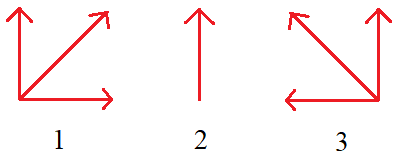
\includegraphics[scale=0.6]{TreForze.png}
    \caption{Forze delle 3 molle e rispettive componenti.}
    \label{TreForze}
\end{figure}
\\
La molla 1 si accorcia di $y\sin(30^\circ)$, determinando una forza $F_{1}=ky\sin(30^\circ)$. La componente verticale di tale forza risulta $F_{1}\sin(30^\circ)=k y\sin^2(30^\circ)$.
\\
La molla 2 si allunga di una quantità $y$, determinando una forza $F_{2}=k y$.
\\
La molla 3 si accorcia di $y\sin(30^\circ)$, la cui forza corrisponde a $F_{3}=k y\sin(30^\circ)$. La componente verticale vale $F_{3}\sin(30^\circ)=k y\sin^2(30°)$.
\\\\
La risultante delle forze delle molle nella direzione \textit {y} è:
\begin{equation}
    |F_m|_y=k y+2k y\sin^2(30^\circ)=1.5k y
\end{equation}
Relativamente agli smorzatori bisognerà fare lo stesso tipo di ragionamento nelle due direzioni del piano oggetto di studio:\\
-lungo \textit {x}
\begin{equation}
    |F_s|_x=2c\dot x\cos^2(30^\circ)=1.5c\dot x
\end{equation}
-lungo \textit {y}
\begin{equation}
    |F_s|_y=c\dot y+2c\dot y\sin^2(30^\circ)=1.5c\dot y
\end{equation}
da cui è possibile ricavare il fattore di smorzamento effettivo del sistema lungo le due direzioni di riferimento, il quale sarà pari a 1.5c.
\\\\
È possibile quindi prendere in considerazione una sola equazione, visto che tutti i coefficienti delle equazioni differenziali del moto in direzione \textit{x} ed \textit{y} sono uguali:
\begin{equation}
    M\ddot y+1.5 c \dot y+1.5k y=me\omega^2  \sin\omega t
    \label{equazionemoto}
\end{equation}
\begin{equation}
    y=Y \sin(\omega t-\psi)
    \label{y}
\end{equation}
\begin{equation}
    \tan\psi=\frac{\frac{2\xi\omega}{\omega_n}}{1-(\frac{\omega}{\omega_n})^2}
\end{equation}
dove M=massa totale sospesa, $\omega_n=\sqrt{\frac{1.5k}{M}}$ pulsazione naturale, $c_{cr}=2\sqrt{1.5kM}$ smorzamento critico e $\xi=\frac{1.5 c}{c_{cr}}$ fattore di smorzamento.
\\\\
L'espressione dell'ampiezza di oscillazione è:
\begin{equation}
    Y=\frac{\frac{me\omega^2}{M\omega_n^2}}{\sqrt{{[1-(\frac{\omega}{\omega_n})^2]^2}+(2\xi \frac{\omega}{\omega_n})^2}}
    \label{Ampiezza}
\end{equation}
Essendo la massa $M$, rappresentativa del cestello, un corpo rigido, tutti i punti appartenenti ad esso si sposteranno nel tempo della stessa quantità $Y$. 
\begin{figure}[h]
    \centering
    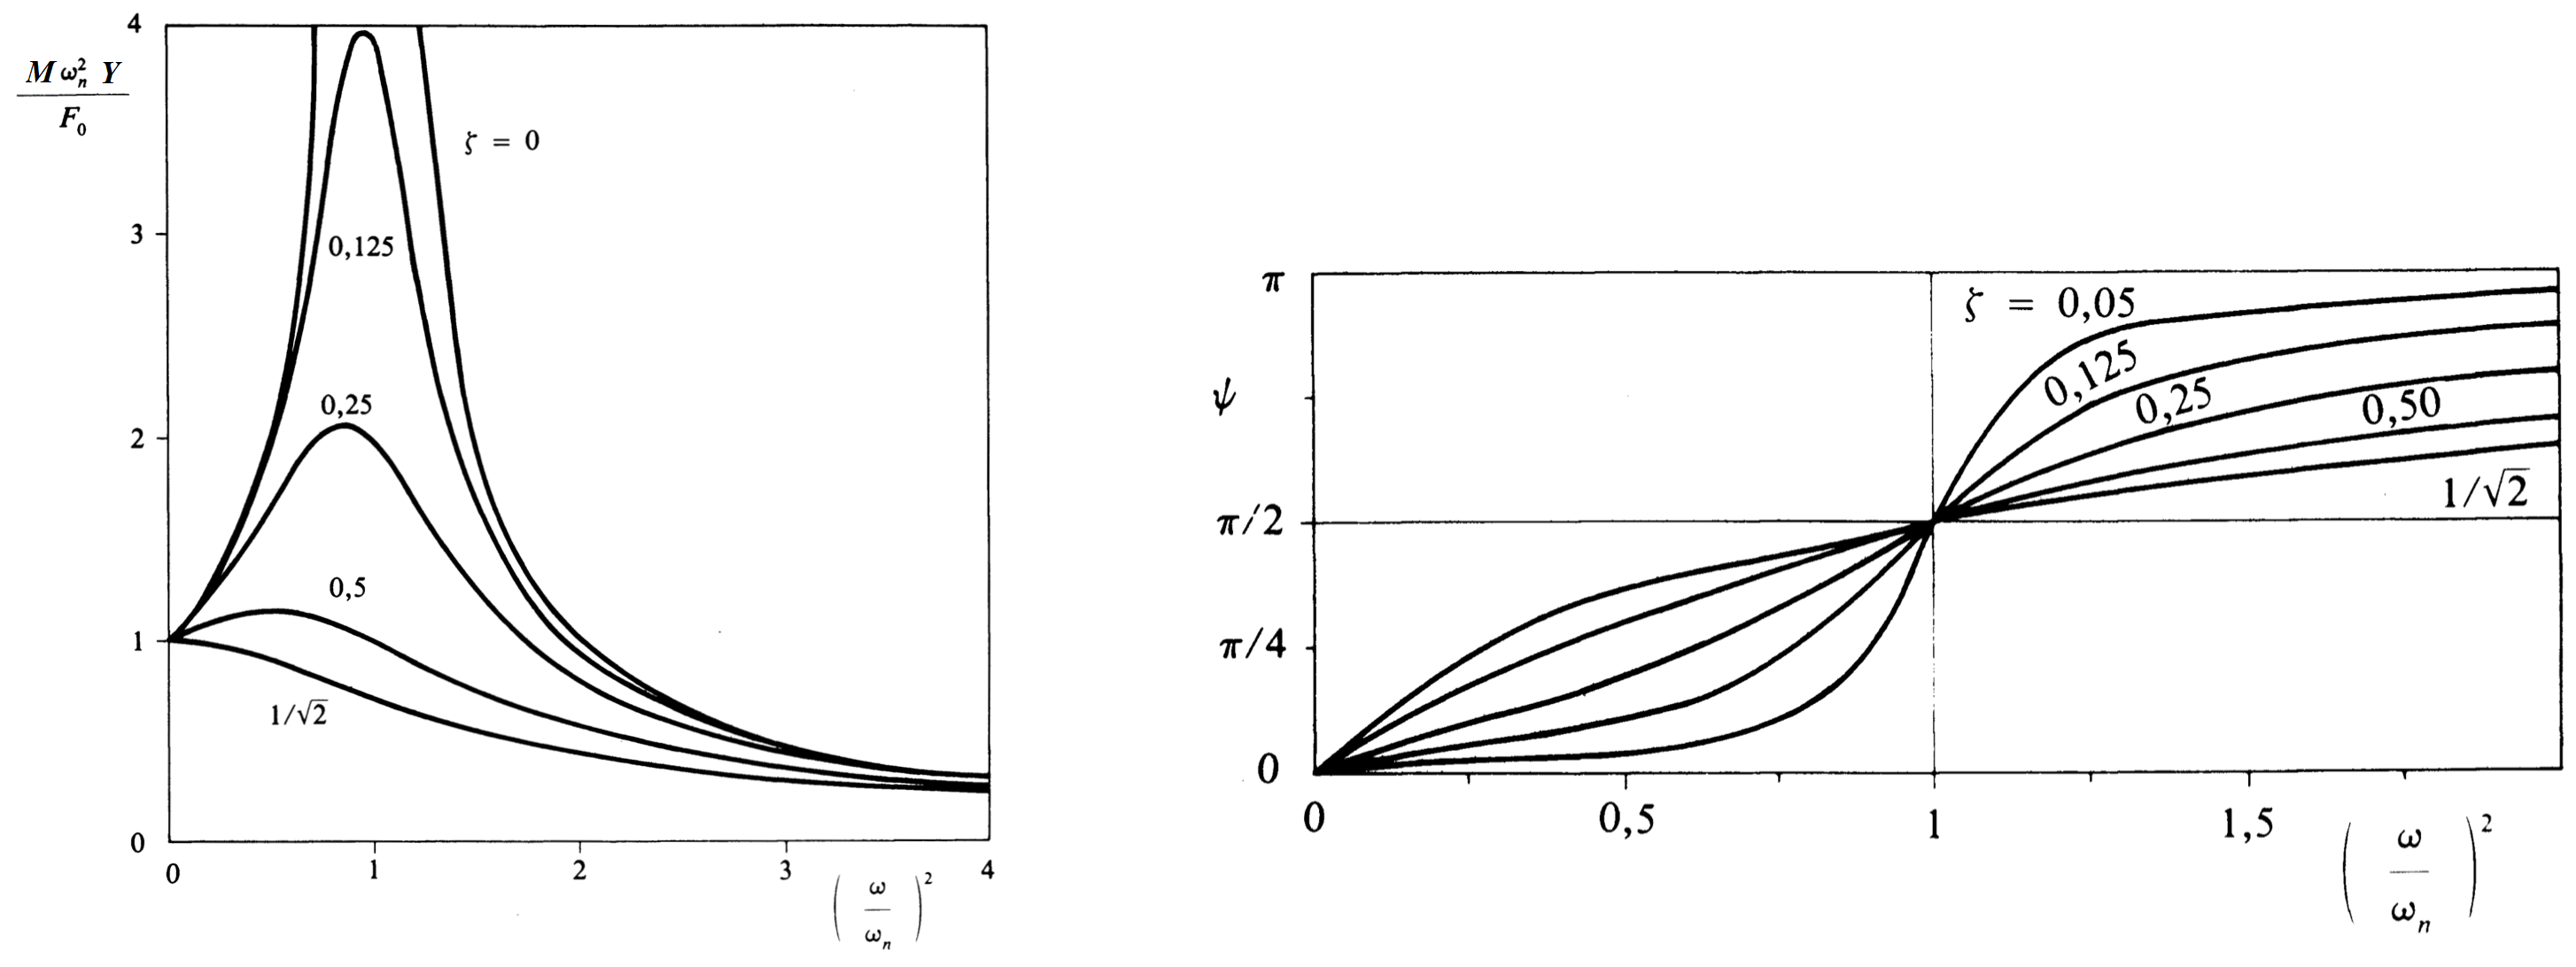
\includegraphics[width=\textwidth]{AmpiezzaEFase.png}
    \caption{Ampiezza e fase della risposta ad una eccitazione sinusoidale di un sistema oscillante ad un grado di libertà.}
    \label{AmpiezzaEfase}
\end{figure}

Lo spostamento $Y_{st}=\frac{F_0}{M\omega_n^2}$ espresso in Figura \ref{AmpiezzaEfase} assume il nome di \textit{spostamento statico}, dove con $F_0$ si è indicato l'ampiezza della forzante. L'ampiezza varia in funzione della pulsazione forzante (rapporto in ascissa). Nei due grafici si possono distinguere tre zone, rispettivamente:
\begin{itemize}
    \item zona quasi statica;
    \item zona di risonanza;
    \item zona sismografica.
\end{itemize}

Il caso oggetto di studio vede una forzante proporzionale al quadrato della pulsazione. Si può quindi riscrivere l'espressione dello spostamento statico come compare in Figura \ref{AmpiezzaEfaseQuadratoDellaPulsazione}, trovando un nuovo andamento grafico.
\begin{figure}[h]
    \centering
    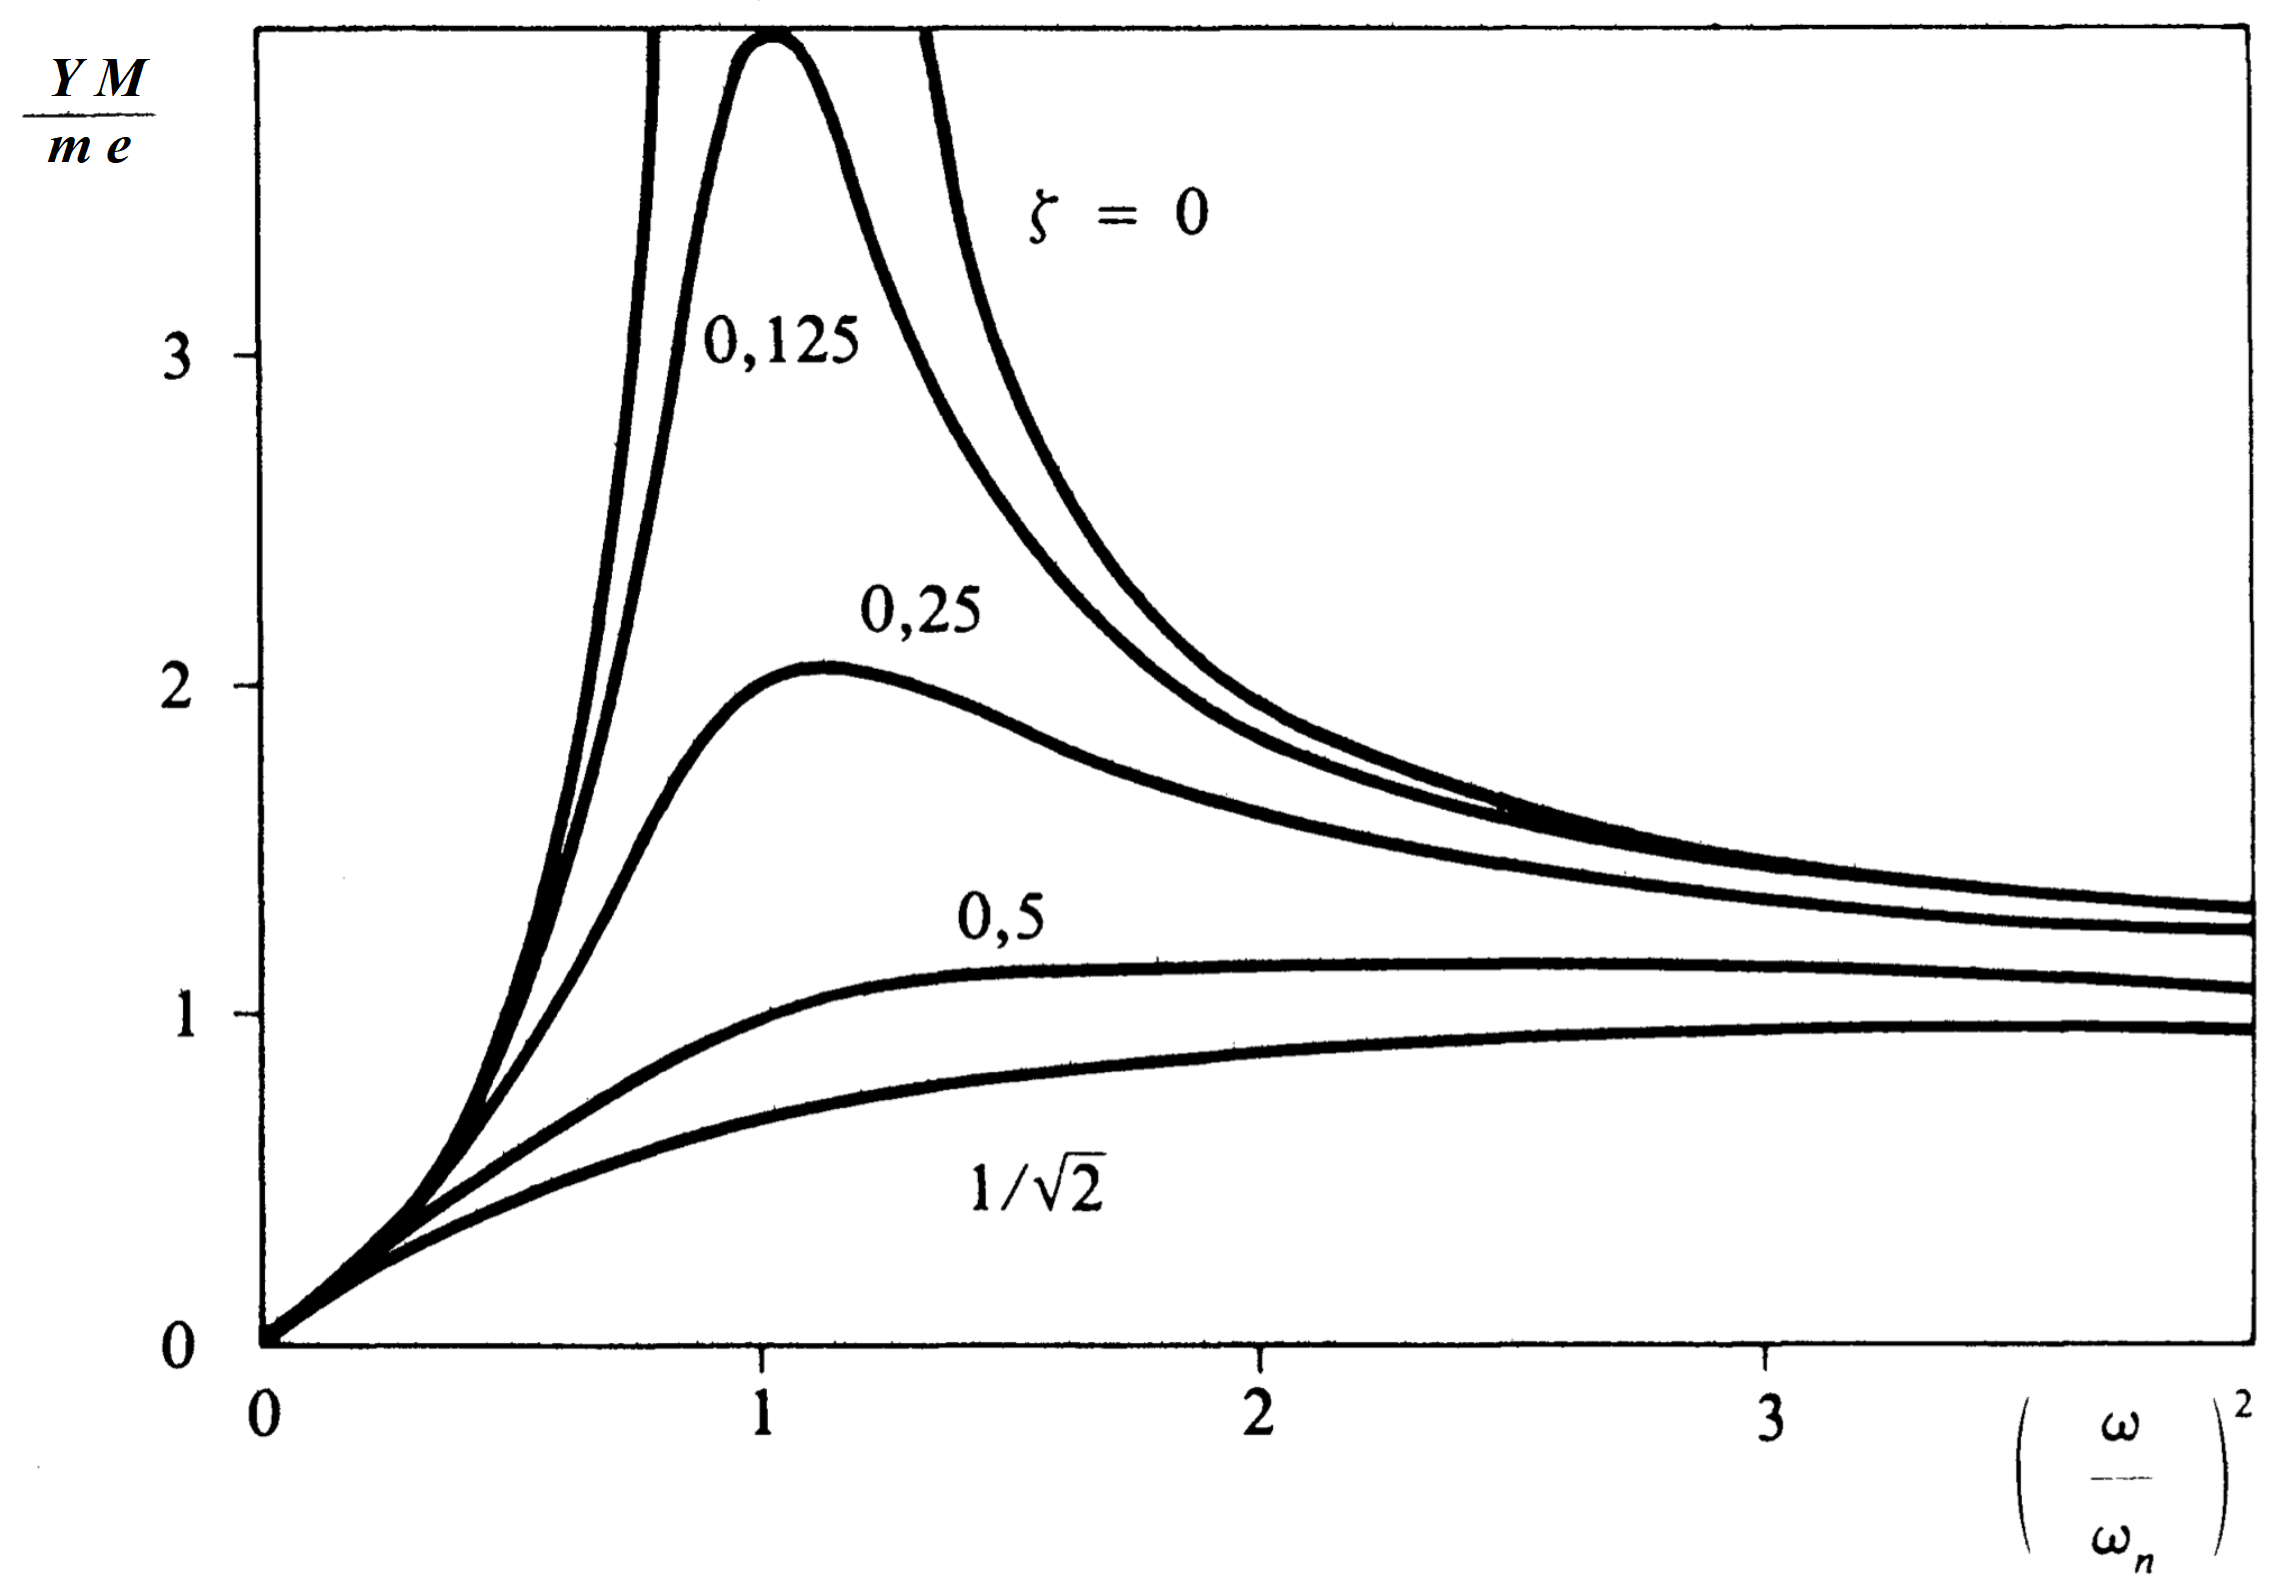
\includegraphics[scale=0.14]{AmpiezzaEfaseQuadratoDellaPulsazione.png}
    \caption{Ampiezza della risposta di un sistema ad un g.d.l. ad una eccitazione sinusoidale con ampiezza proporzionale al quadrato della pulsazione.}
    \label{AmpiezzaEfaseQuadratoDellaPulsazione}
\end{figure}
\subsection{Trasmissibilità al telaio}
Sul telaio della lavatrice agisce una forza eccitatrice periodica come nel caso precedente. Tale forza prende l'espressione \begin{equation}
    T=k y+c \dot y.
\end{equation}
Inserendo all'interno l'espressione (\ref{y}), diventa
\begin{equation}
    T=Y\left[k\sin (\omega t -\psi)+c \omega\cos(\omega t-\psi)\right].
\end{equation}
Essendo $T$ somma di due funzioni sinusoidali di pulsazione $\omega$, sarà anch'essa una funzione sinusoidale della medesima pulsazione. Più in dettaglio, può essere pensata come proiezione su una retta di una forza costante $T_0$, rotante con velocità angolare $\omega$ attorno ad un asse perpendicolare alla sua retta d'azione. 

Anche le due forze al secondo membro possono essere pensate come proiezioni di forze rotanti con velocità angolare $\omega$, sfasate tra loro di $\pi/2$ e di ampiezze $k Y$ e $c\omega Y$.

Per il teorema di Pitagora si ottiene
\begin{equation}
    T_0=Y\sqrt{k^2+c^2\omega^2}.
\end{equation}
Rielaborando con le espressioni di $\omega_n$, $\xi$ e le notazioni precedenti si ottiene:
\begin{equation}
    T_o=M\omega_n^2Y\sqrt{1+(2\xi \frac{\omega}{\omega_n})^2}
\end{equation}
Una volta sostituita l'espressione di Y:
\begin{equation}
  \tau =  \frac{T_o}{me\omega^2}=\frac{\sqrt{1+(2\xi \frac{\omega}{\omega_n})^2}}{\sqrt{[1-(\frac{\omega}{\omega_n})^2]^2+(2\xi\frac{\omega}{\omega_n})^2}}
\end{equation}
si ottiene un'espressione significativa dell'efficacia della trasmissione della forza al telaio, detta \textit{trasmissibilità} ($\tau$).
\begin{figure}[h]
    \centering
    \includegraphics[scale=0.2]{trasmissibilità.png}
    \caption{Andamento della trasmissibilità per diversi valori di $\xi$.}
    \label{trasmissibilità}
\end{figure}
In presenza del nodo (Figura \ref{trasmissibilità}) la forza applicata è uguale alla forza trasmessa, quindi conviene lavorare in zona sismografica. $\tau$ è pari all'unità per qualsiasi valore di $\xi$, sia per $\omega/\omega_n=0$ che per $\omega/\omega_n=2$. Il rapporto risulta minore di 1 per $(\omega/\omega_n)^2>2$, campo nel quale la sospensione risulta efficace. La sua efficacia è tanto maggiore, quanto più è grande $\omega/\omega_n$, ovvero quanto più la sospensione è cedevole \cite{meneghetti2010lezioni}.
\subsection{Lavoro dissipato}
E' noto che il lavoro svolto dalla forza d'inerzia e da quella elastica nell'arco di un periodo è sempre nullo. Chiameremo allora $L_p$ il \textit{lavoro dissipato} a causa dell'attrito viscoso:
\begin{equation}
    L_p=\int_{0}^{T}c\dot x\dot x dt=\int_{0}^{T}c\omega^2 X^2 \sin^2(\omega t-\psi)dt=\pi c\omega X^2
\end{equation}
 Quest'ultimo, nelle condizioni di regime, è uguale al lavoro svolto dalla forza eccitatrice.